\documentclass[12pt,letterpaper]{article}
\usepackage[utf8]{inputenc}
\usepackage[left=2cm,right=2cm,top=2cm,bottom=2cm]{geometry}
\usepackage{multirow}
\title{Informe Oracle}
\author{Juan Rodriguez}
\date{November 2018}



\usepackage{graphicx}

\begin{document}
    
    \begin{center}
        
\includegraphics[width=4cm]{Imagenes/upt-logo.png}\\
        \vspace{12pt}
        \vspace{12pt}
        \large\textbf{UNIVERSIDAD PRIVADA DE TACNA}\\
        \vspace{12pt}
        \vspace{12pt}
        \large{FACULTAD DE INGENIERIA}\\
        \vspace{12pt}
        \vspace{12pt}
        \large{Escuela Profesional de Ingeniería de Sistemas}\\
        \vspace{12pt}
        \vspace{12pt}
        \textbf{INFORME LABORATORIO 6}\\
        \vspace{12pt}
        \vspace{12pt}
        Curso: Bases de Datos II\\
        \vspace{12pt}
        Docente: Ing. Patrick Cuadros\\
        \vspace*{12pt}
           \begin{flushleft}
        Alumno:\\
        \vspace{12pt}
        Rodriguez Mamani, Juan Rigoberto\hfill (2017057862)\\

        \end{flushleft}
        \vspace{100pt}

        Tacna – Perú\\
            2018
        \vspace{12pt}

            \thispagestyle{empty} % CARATULA SIN NUMERO
            \setcounter{page}{0} % REINICIAR CONTADOR DE PAGINAS
    \end{center}
    \break

\section{Cuestionario}
\vspace{12pt}

\subsection{¿Qué sucede al ejecutar los siguientes comandos?}
\vspace{12pt}
\textbf{STARTUP OPEN:} Abre la base de Datos de Oracle.
\vspace{10pt}\\
\textbf{STARTUP MOUNT:} Monta la base de datos pero no lo abre.
\vspace{10pt}\\
\textbf{STARTUP NOMOUNT:} Hace que la base de datos no se monte al iniciar la instancia.
\vspace{10pt}\\
\textbf{STARTUP FORCE:} Cierra la instancia actual de la base de datos Oracle (si se está ejecutando) con el modo APAGADO ABORTADO, antes de reiniciarlo. Si la instancia actual se está ejecutando y FORCE no está especificado, se produce un error. FORCE es útil para la depuración y en circunstancias anormales. Normalmente no se debe utilizar.
\vspace{10pt}\\
\textbf{STARTUP RESTRICT:} Permite a los usuarios de Oracle Database con el privilegio del sistema RESTRICTED SESSION conectarse a la base de datos. Más adelante, puede usar el comando ALTER SYSTEM para deshabilitar la función de sesión restringida.
\vspace{10pt}\\
\textbf{STARTUP RECOVER:} Especifica que la recuperación de medios se debe realizar, si es necesario, antes de iniciar la instancia. STARTUP RECOVER tiene el mismo efecto que emitir el comando RECOVER DATABASE e iniciar una instancia. Solo la recuperación completa es posible con la opción RECOVER.
\vspace{10pt}\\
\textbf{SHUTDOWN NORMAL:} NORMAL es la opción por defecto que espera a que los usuarios se desconecten de la base de datos. Otros enlaces están prohibidos. La base de datos está cerrada y desmontada. La instancia se apaga y no se requiere ninguna recuperación de instancia en el próximo inicio de la base de datos.
\vspace{10pt}\\
\textbf{SHUTDOWN TRANSACTIONAL:} Realiza un cierre planificado de una instancia mientras permite que las transacciones activas se completen primero. Evita que los clientes pierdan el trabajo sin que todos los usuarios se desconecten. Ningún cliente puede iniciar una nueva transacción en esta instancia. Intentar iniciar una nueva transacción da como resultado la desconexión. 
\vspace{10pt}\\
\textbf{SHUTDOWN ABORT:} Continúa con el cierre más rápido posible de la base de datos sin esperar a que las llamadas se completen o los usuarios se desconecten. Las transacciones no confirmadas no se retrotraen. Las instrucciones SQL del cliente que se están procesando actualmente se terminan. Todos los usuarios actualmente conectados a la base de datos están desconectados implícitamente y el próximo inicio de la base de datos requerirá la recuperación de la instancia.
\vspace{10pt}\\
\textbf{SHUTDOWN INMEDIATE:} No espera a que se completen las llamadas actuales o que los usuarios se desconecten de la base de datos. Otros enlaces están prohibidos. La base de datos está cerrada y desmontada. La instancia se apaga y no se requiere ninguna recuperación de instancia en el próximo inicio de la base de datos.\\
\break


\subsection{En el script lab\_02\_01.sql, se establecen privilegios de sistema, enliste los privilegios de sistema (DDL) utilizados y describa cada uno de ellos.}
\vspace{12pt}
\begin{center}
  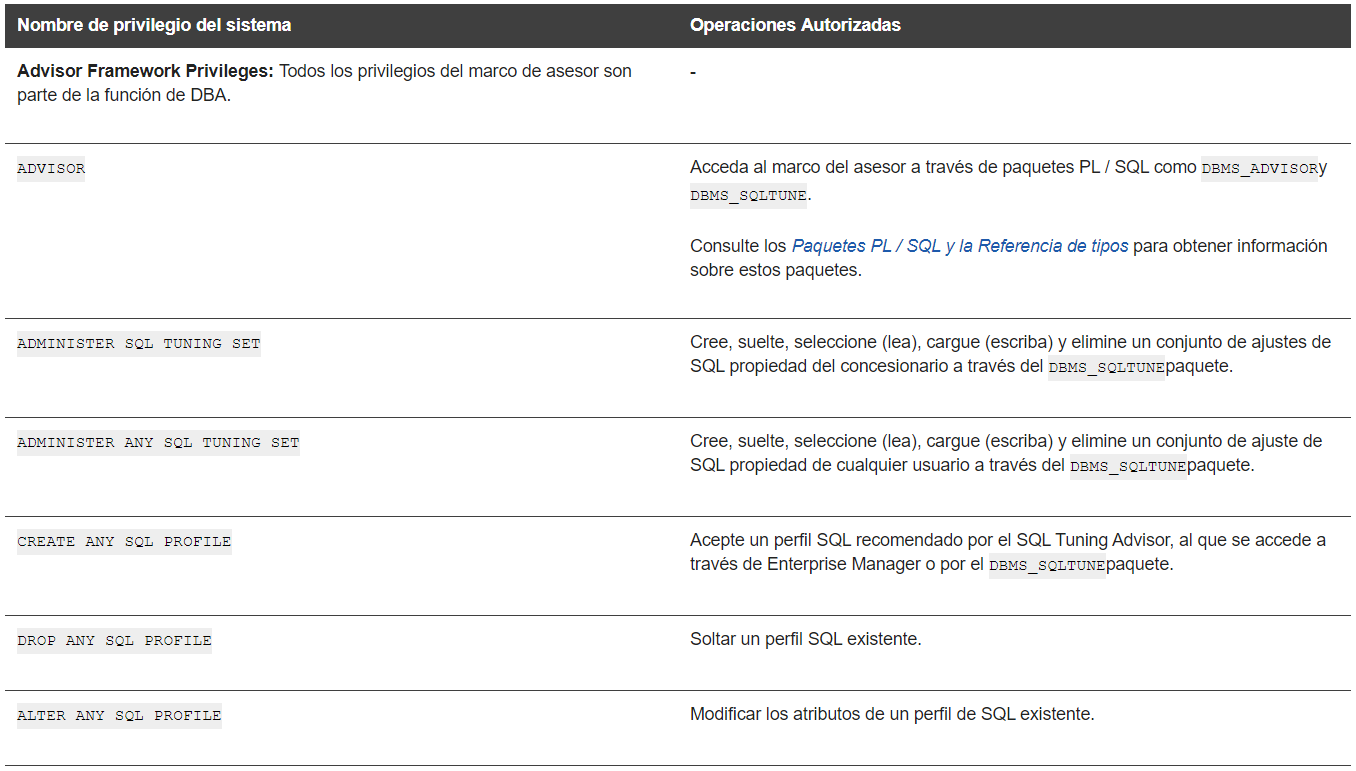
\includegraphics[width=14cm]{Imagenes/Privilegios_sistema.png}\\
\end{center}

\begin{center}
  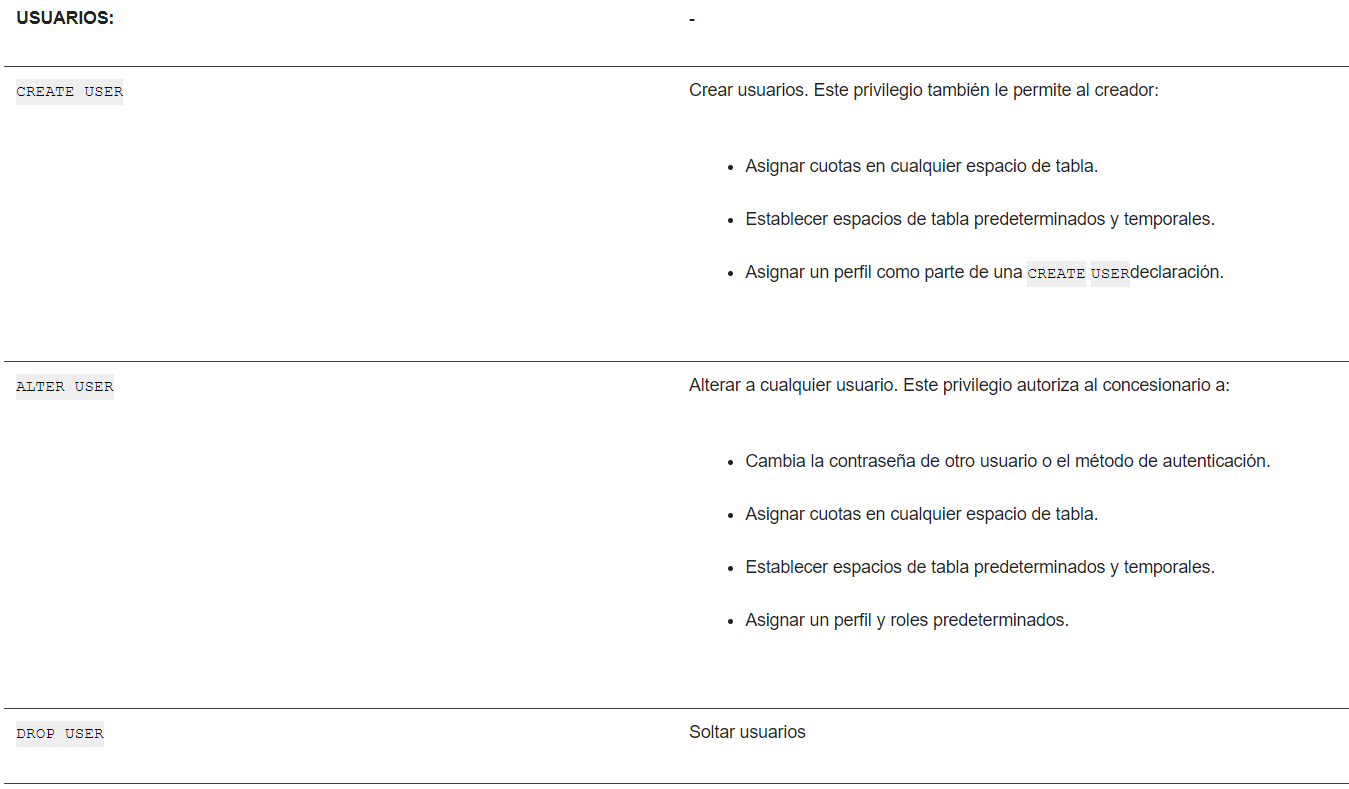
\includegraphics[width=14cm]{Imagenes/Privilegios_usuarios.png}\\
\end{center}

\begin{center}
  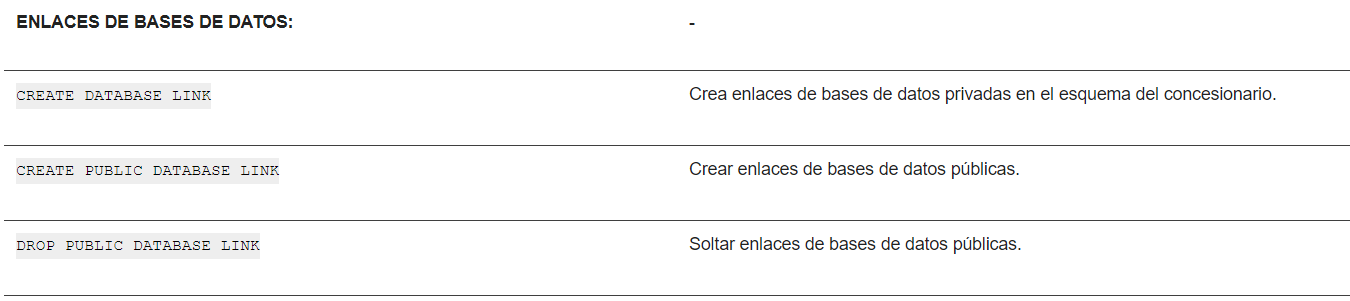
\includegraphics[width=14cm]{Imagenes/Privilegios_basedatos.png}\\
\end{center}
\break
\begin{center}
  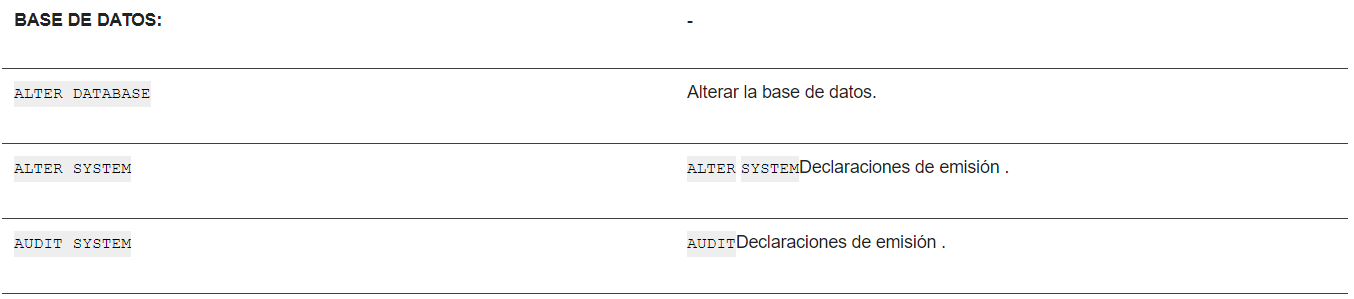
\includegraphics[width=14cm]{Imagenes/Privilegios_datos.png}\\
\end{center}

\begin{center}
  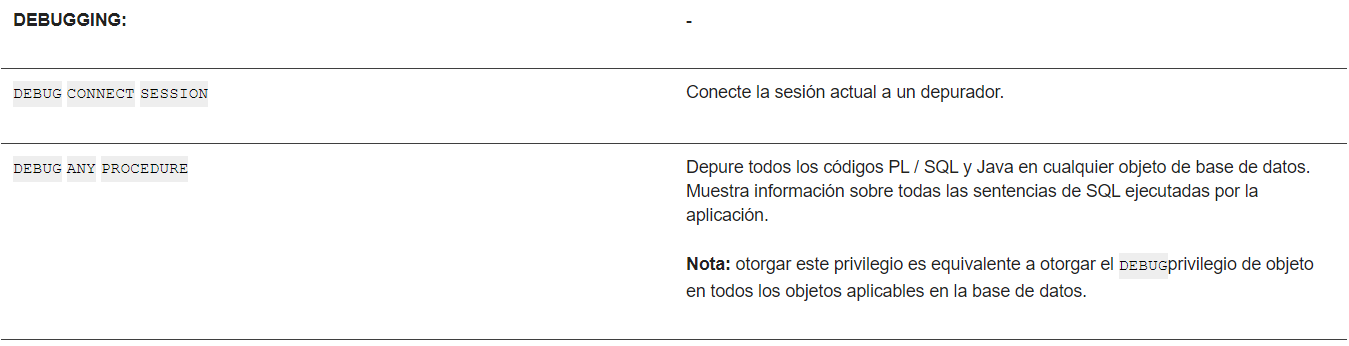
\includegraphics[width=14cm]{Imagenes/Privilegios_debugging.png}\\
\end{center}

\begin{center}
  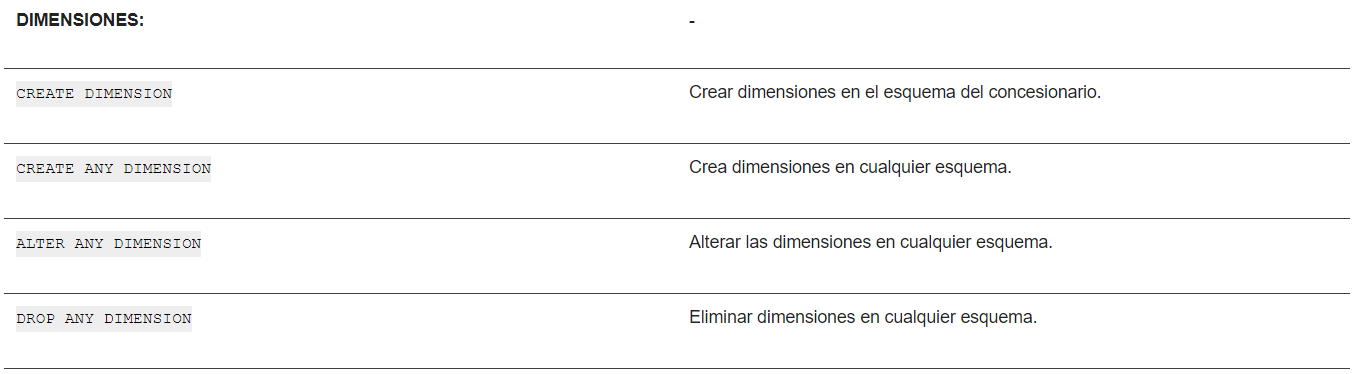
\includegraphics[width=14cm]{Imagenes/Privilegios_dimensiones.png}\\
\end{center}

\begin{center}
  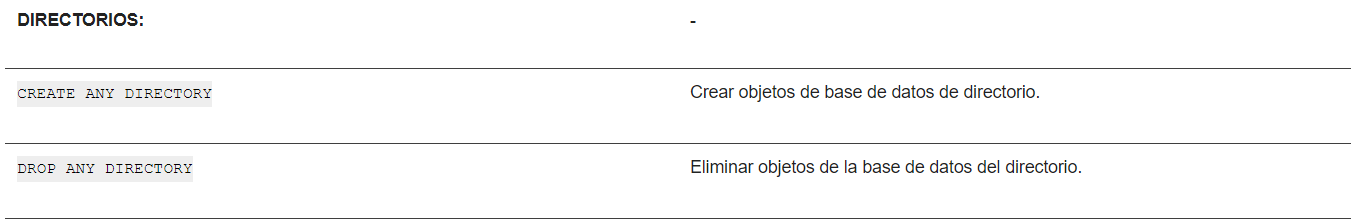
\includegraphics[width=14cm]{Imagenes/Privilegios_directorios.png}\\
\end{center}

\begin{center}
  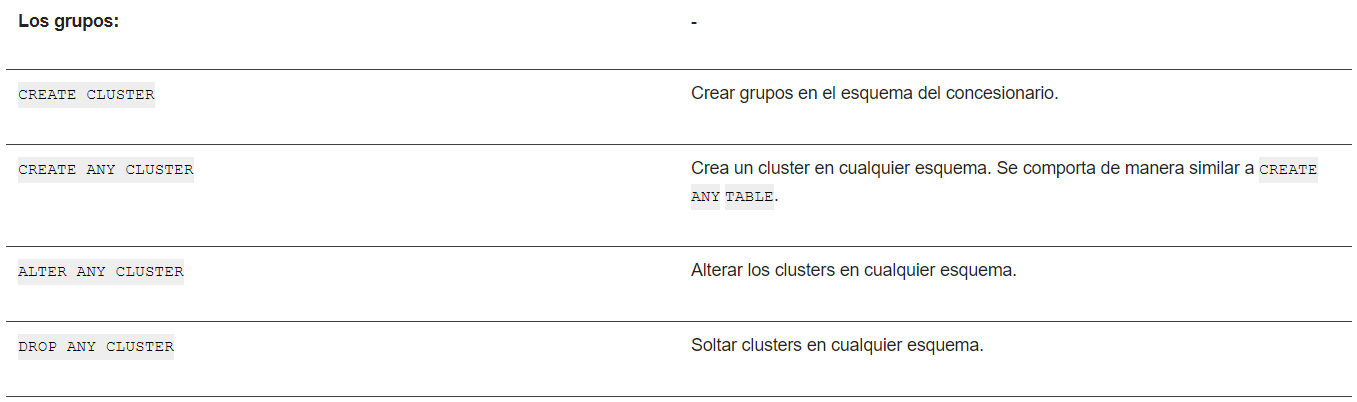
\includegraphics[width=14cm]{Imagenes/Privilegios_grupos.png}\\
\end{center}

\begin{center}
  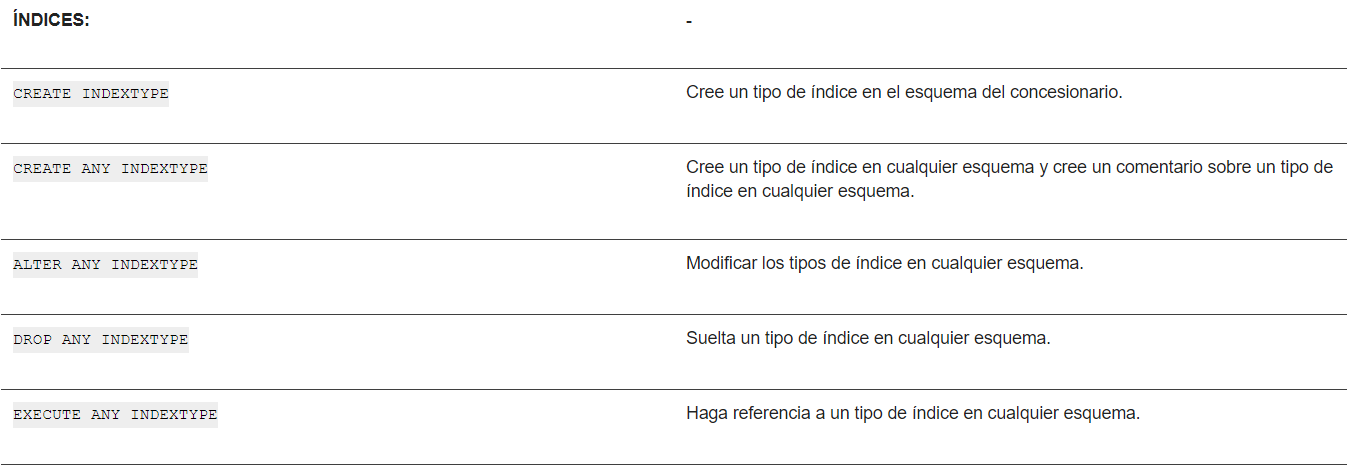
\includegraphics[width=14cm]{Imagenes/Privilegios_indices.png}\\
\end{center}

\begin{center}
  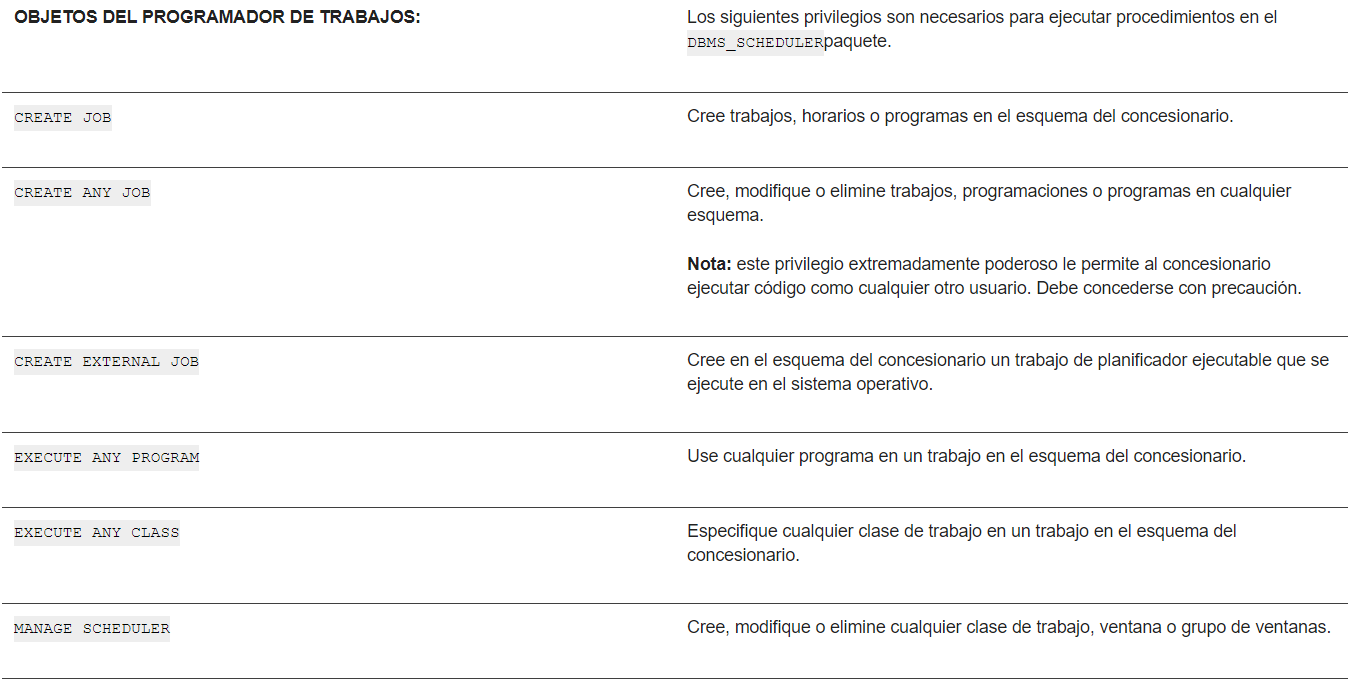
\includegraphics[width=14cm]{Imagenes/Privilegios_objetosprogramador.png}\\
\end{center}

\begin{center}
  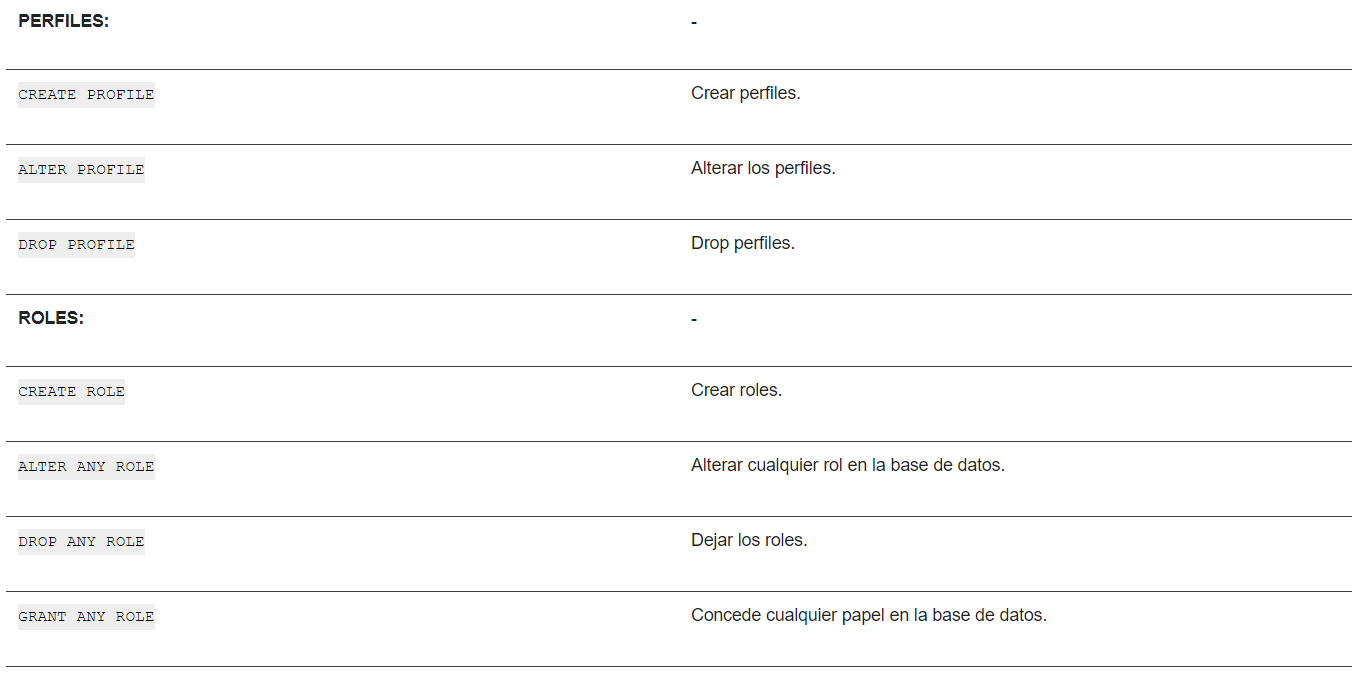
\includegraphics[width=14cm]{Imagenes/Privilegios_perfilesroles.png}\\
\end{center}

\begin{center}
  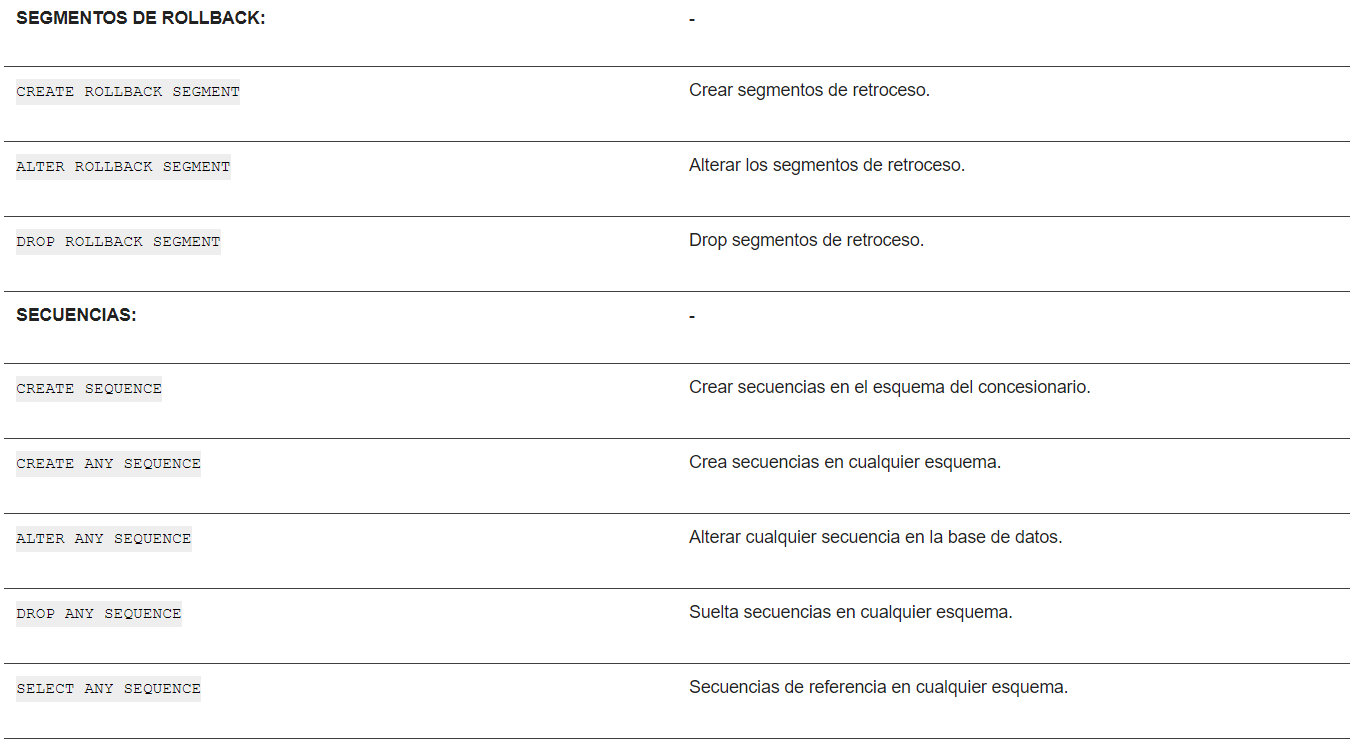
\includegraphics[width=14cm]{Imagenes/Privilegios_segmentossecuencias.png}\\
\end{center}

\begin{center}
  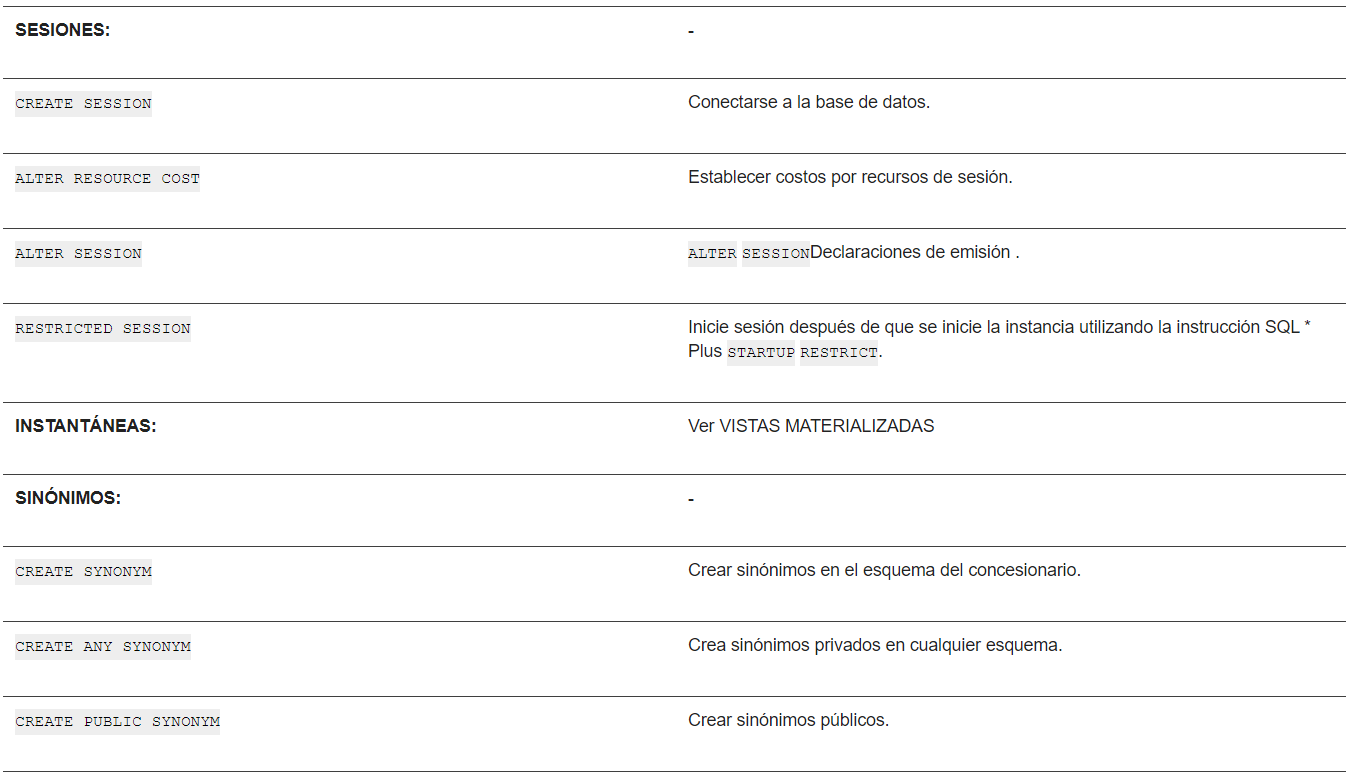
\includegraphics[width=14cm]{Imagenes/Privilegios_sesionessinonimos.png}\\
\end{center}

\begin{center}
  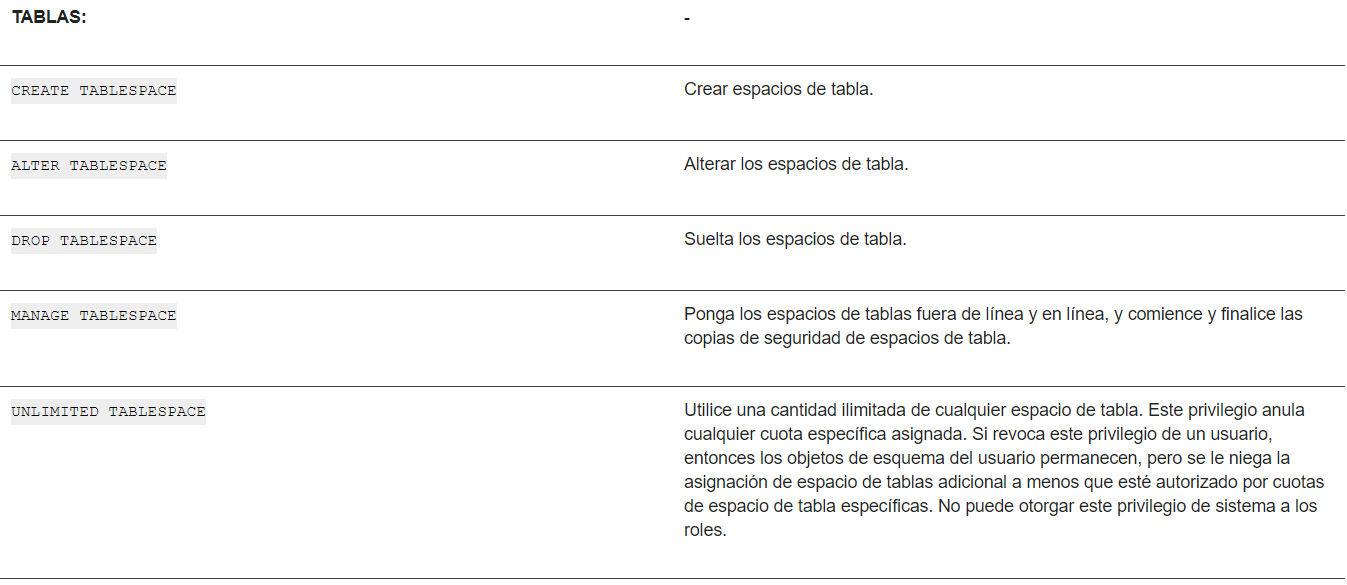
\includegraphics[width=14cm]{Imagenes/Privilegios_tablas.png}\\
\end{center}

\begin{center}
  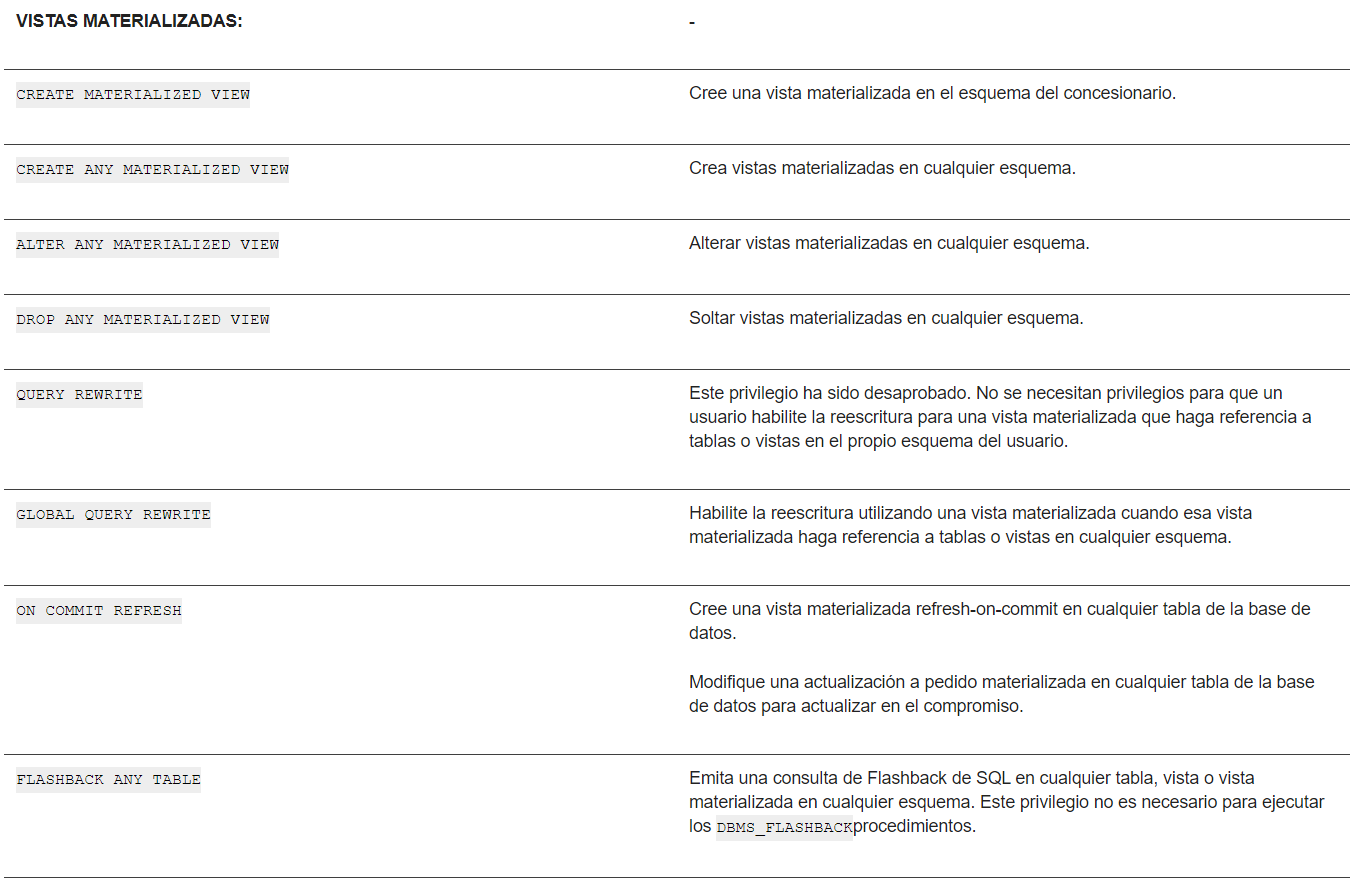
\includegraphics[width=14cm]{Imagenes/Privilegios_vistasmaterializadas.png}\\
\end{center}
\subsection{Enliste y describa los tipos de TableSpace que existen en Oracle.}
\vspace{12pt}
Existen 3 tipos de TableSpace en Oracle:
\vspace{10pt}\\
\textbf{PERMANENT (Permanente):} Utiliza espacios de tabla permanentes para almacenar sus datos de usuario y aplicación. La base de datos Oracle utiliza espacios de tabla permanentes para almacenar datos permanentes, como los datos del sistema. A cada usuario se le asigna un espacio de tabla permanente predeterminado.
\vspace{10pt}\\
\textbf{UNDO (Deshacer):} Una base de datos que se ejecuta en el modo de administración automática de deshacer crea y administra de forma transparente los datos de deshacer en el espacio de tablas de deshacer. La base de datos Oracle utiliza los datos de deshacer para revertir las transacciones, para proporcionar coherencia de lectura, para ayudar con la recuperación de la base de datos y para habilitar funciones como Oracle Flashback Query. Una instancia de base de datos solo puede tener un espacio de tablas de deshacer activo.
\vspace{10pt}\\
\textbf{TEMPORARY (Temporal):} Los espacios de tabla temporales se utilizan para almacenar datos temporales, como se crearía cuando las sentencias de SQL realicen operaciones de clasificación. Una base de datos Oracle obtiene un espacio de tabla temporal cuando se crea la base de datos. Si estuviera creando un grupo de espacio de tablas temporal, crearía otro espacio de tabla temporal. En circunstancias típicas, no es necesario crear espacios de tabla temporales adicionales. Si tiene una base de datos extremadamente grande, entonces puede configurar espacios de tabla temporales adicionales.
Los archivos físicos que comprenden un espacio de tabla temporal se denominan archivos temporales, a diferencia de los archivos de datos.
\vspace{10pt}\\


\end{document}